\documentclass[11pt]{article}

\usepackage{fullpage}
\usepackage{booktabs}
\usepackage{graphicx}

\def\rootdir{../}

\begin{document}

\section*{Lecture outline -- Safety engineering}

{\bf Learning outcomes:} 

 \begin{enumerate}
  
  \item Define the term ``safety'' as it related to software and systems, and demonstrate the difference between safety and other qualities, such as correctness and reliability.

  \item Understand the high-level process used for safety engineering.

  \item Explain how accidents relate to and influence safety engineering.

  \item Use an event chain to describe an accident.

  \item Explain the concepts of risk, integrity, hazard, accident, and causation.

  \item Apply HAZOPS to identify preliminary hazards.

  \item Apply FMEA to analyse the safety concerns of a design.

  \item Apply fault-tree analysis to a design.

 \end{enumerate}

\section*{Lecture plan}

\textbf{Safety and accidents}

\begin{enumerate}

 \item Define \emph{safety} and how it differs to correctness, reliability, etc. A product is safe if it does not cause unacceptable harm or damage; e.g. to a person or to the environment.

 \item NOTE: Safety must be considered outside of the boundaries of the software --- software alone cannot harm anything.

 \item Examples of failures:

  \begin{description}

    \item[Therac-25]  -- Between June 1985 and January 1987, six people died after receiving more than 100 times the intended radiation dose from Therac-25 radiation therapy machine. Investigation concluded \emph{poor software design}.

   \item[A320 Airbus Accidents] -- The Lufthansa A320 accident at
      Warsaw airport, and the Mulhouse-Habsheim Airport accident (discussed in more detail below).

    \item[London Ambulance] -- October 1992, the failure CAD system resulted in over 30 deaths and problems in dealing with life-threatening incidents. Up to 11 hours of waiting. Investigation concluded poor design and implementation.

  July 2006 upgrade: repeated crashes, so back to pen and paper methods.

  June 2011 new system: developed tech problems, so back to pen and paper methods, and revert to previous system on the same day. Not re-instated until May 2012.

  \end{description}

 \item  A320 Airbus: a \emph{fly by wire} aircraft, described a \emph{``network with an aircraft wrapped  around it''}. 150 ECUs.

 \item  Mulhouse-Habsheim Airport accident (France):

  \begin{enumerate}

  \item Demonstration of the aircraft's capability at low  altitude.

  \item First demo at 10m with landing gear down, second demo at 30m without landing gear. 

  \item Crashed during second demo, killing 3 of the 130 passengers and injuring 34 others.

 \item Investigation: low fly-over, low speed (flight idle), late application of thrust, no malfunction $\rightarrow$ \emph{pilot error}.

 \item Observation: pilot error far more likely to be concluded when pilot dies (not there to defend themselves).

 \item If pilot e.g.\ does not notice a signal, is this entirely the pilot's fault, or is the greater system to blame?

 \item Back to Habsheim --- pilot's version: 

  \begin{enumerate}

   \item company procedures not followed (by others): fly-over lower than specified, flight dossier about airport arrived too late for crew to study; trees 30-40ft high not known about until 15 seconds away.

   \item Altimeter faulty: displays 67ft before take off.

  \item Runway shorter than normal runway -- had never landed at this airport before..

  \end{enumerate}

  \item Technical problems: two guidance systems, not communicating as they should. Caused problems, so entered data into only one.

  \item Pilot claims engines took almost 9 seconds to spool rather than 5 seconds they should.

 \item Conclusion: accident cause is system-wide: bad reporting, fault systems, procedures not followed, unexpected environment, and \emph{maybe} some pilot error.

  \end{enumerate}


 \item Accidents in safety: accidents and incidents are the most useful way to identify potential hazard. By looking at older systems in the same domain, we can get an idea of the factors that contributed to accidents and incidents.

 \item Causality: \emph{When can it be said that event A causes event B}?:

 \begin{enumerate}

  \item Reason with \emph{counterfactuals}: what could have happened under different conditions.

  \item Example (and hint): ``They would have done better on their assignments, if they had first done the workshops'

  \item For accidents, ``{\em A causes B}'' if we assume that {\em A}
did not occur then {\em B} would not have occurred. 

  \item NOTE: this makes event \emph{A} just \emph{one} cause, not (necessarily) the sole cause.

  \item Be careful not to confuse counterfactuals with correlation: \emph{If the were the case that the barometer falls then a storm would occur.}

 \end{enumerate}

\end{enumerate}

\textbf{Safety engineering}

\begin{enumerate}

 \item Three relevant phases in a SE lifecycle:

  \begin{enumerate}

   \item \emph{preliminary hazard analysis}: identify what can go wrong (hazards).

   \item \emph{design}: design the system to mitigate the hazards.

   \item \emph{implement and test}: implement the design correctly.

  \end{enumerate}

  \item PHA: input is system data and previous accident info. Method is to brainstorm. Output is a \emph{hazard log}: lists the hazards, their causes and their  severity,  as well as other data such as target frequencies or hazard types.

  \item Show risk \& frequency values, and their classes (below).

\end{enumerate}

\textbf{HAZOPS}

\begin{enumerate}

 \item \emph{Exploratory} hazard analysis. Well established and used.

 \item Basic outline: take intended behaviour of a single design item, vary that behaviour, and brainstorm what could happen. Group brainstorming with domain experts who know a lot about accidents.

 \item Example: brake by wire system in a vehicle. Used by Mercedes Benz and Toyota in most new vehicles. Intended behaviour: push brake and car slows down. Chain is brake pedal $\rightarrow$ ECU $\rightarrow$ braking actuator. HAZOP:

   Get class to do NONE, EARLY, and LATE signals.

 \item Record: deviation (guideword + design item), causes, consequences, safeguards in place, and list of recommendations.

  Show guideword table in appendix of this sheet.

 \item Limitations: needs some described behaviour (so may come late in process), time and resource intensive, documentation heading, focuses on single failures.

\end{enumerate}

\textbf{Fault tree analysis}

\begin{enumerate}

 \item A \emph{deductive} technique: starts with potential hazards and works backwards, trying to determine what could cause them. Done on design, not requirements.

 \item Symbols (see below).

 \item Identify \emph{immediate}, \emph{necessary} (linked with AND), and \emph{sufficient} (linked with OR) events.

 \item Example: chemical mixing plant.

\end{enumerate}

\textbf{FMEA -- Failure modes and effects analysis}

\begin{enumerate}

  \item An \emph{inductive} technique: starts with a failure mode and works forward to the consequence, using the system design. It is about identifying the \emph{failure modes} of the system.

  \item Typical failure modes are: 

  \begin{enumerate}
  \item Premature operation.
  \item Failure to operate at the required time.
  \item Failure to stop operation at the required time.
  \item Failure during operation --- and this is specific to the equipment.
  \item Degraded operational capacity.
  \item Excessive operational capacity.
  \end{enumerate}

 \item Method: need a solid definition of the system.

 \item Method: step 1 --- what are the failure modes?

 \item Method: step 2 --- what are the failure effects?

 \item Result: worksheet, documenting failure modes and effects, along with other items, such as causes, probabilities, severities, and recommendations. 

 \item Limitations: individual failures only (not chains), time and resource intensive, sometimes FMEA is done only to satisfy the altruistic urge  to ``do safety'' (\emph{How will the results be used?}).

\end{enumerate}

\pagebreak

\section*{IEC  61508 standard}


\subsubsection*{Risks}
      \begin{center}
            \begin{tabular}{ll} 
              catastrophic & critical \\
              marginal     & negligible
            \end{tabular}
        \end{center}

\subsubsection*{Frequencies}
        \begin{center}
            \begin{tabular}{lll}
                frequent & probable & occasional \\
                remote   & improbable & incredible
            \end{tabular}
        \end{center}

\subsubsection*{Risk classes}

\begin{center}
    \begin{tabular}{lcccc}
	\toprule
	Frequency & \multicolumn{4}{c}{Consequence}\\\cmidrule{2-5}
                  & Catastrophic & Critical & Marginal & Negligible \\
	\midrule
	Frequent & I & I & I & II \\
	Probable & I & I & II & III\\
	Occasional & I & II & III & III\\
	Remote & II & III & III & IV \\ 
	Incredible & IV & IV & IV & IV \\
	\bottomrule
    \end{tabular}
\end{center}

\begin{tabular}{ll}

\textbf{Class I} & Intolerable risk.\\

\textbf{Class II} & Undesirable risk and tolerable only if risk
	  	reduction is impractical.\\

\textbf{Class III} & Tolerable risk if the cost of risk reduction
		would exceed the improvement gained.\\

\textbf{Class IV} & Negligible risk.

\end{tabular}

\pagebreak


\begin{center}
\begin{tabular}{lp{11cm}}
 \multicolumn{2}{c}{{\Large \textbf{HAZOPS guidewords}}}\\[2mm]
 \toprule
      \textbf{Guide Word} & \textbf{Deviation}\\
 \midrule
      NO or NONE & This is the complete negation of the design intention. No
      part of the intention is achieved and nothing else happens.\\
      MORE & This is a quantitative increase.\\
      LESS & This is a quantitative decrease.\\
      AS WELL AS & All the design intention is achieved together with additions.\\
      PART OF & Only some of the design intention is achieved. \\
      REVERSE & The logical opposite of the intention is achieved.\\
      OTHER THAN & Complete substitution, where no part of the original
      intention is achieved but something quite different happens. \\
    EARLY  & Something happens earlier than expected relative to clock time.\\
    LATE & Something happens later than expected relative to clock time. \\
    BEFORE & Something happens before it is expected, relating to
    order or sequence.\\
    AFTER & Something happens after it is expected, relating to order or sequence.\\
\bottomrule
\end{tabular}
\end{center}

\pagebreak

\section*{Fault tree symbols}

\begin{center}
  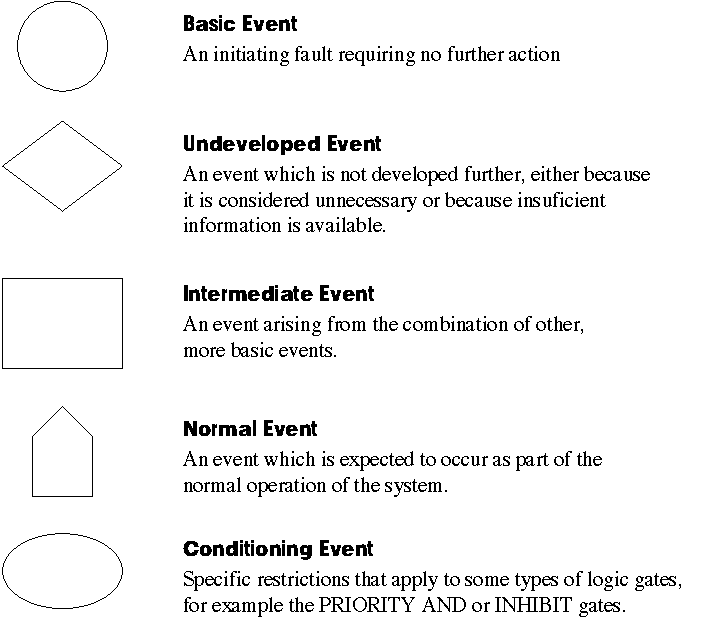
\includegraphics[scale=0.8]{\rootdir/safety/figures/fault-tree-symbols}
\end{center}

\begin{center}
  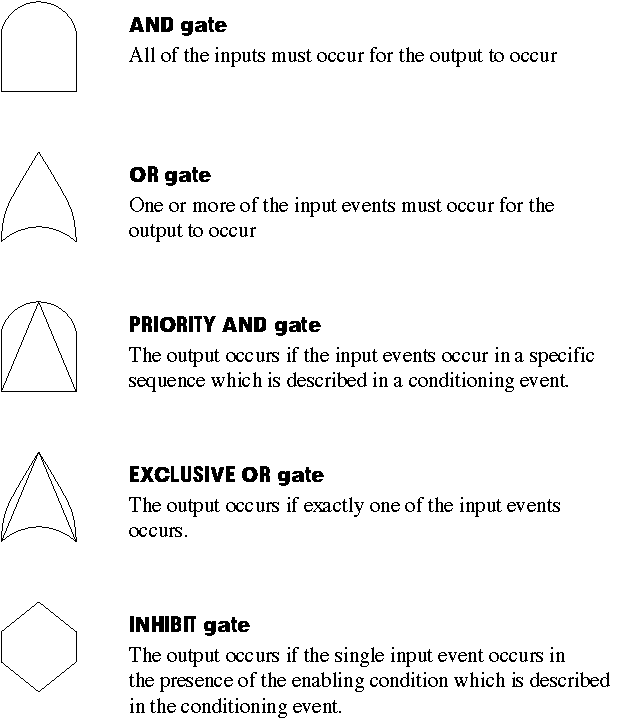
\includegraphics[scale=0.8]{\rootdir/safety/figures/fault-tree-gates}
\end{center}


\pagebreak

\section*{Fault tree example}

\begin{center}
  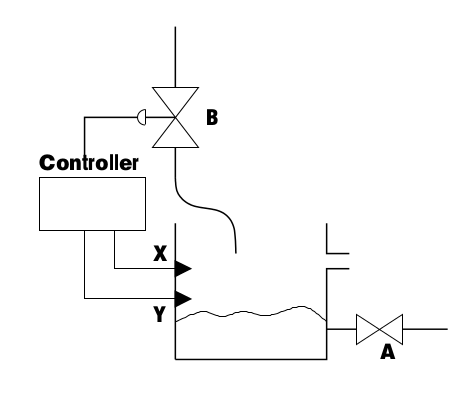
\includegraphics[scale=0.8]{\rootdir/safety/figures/chemical-mixing}
\end{center}

\pagebreak

\section*{Fault tree example}

\begin{center}
  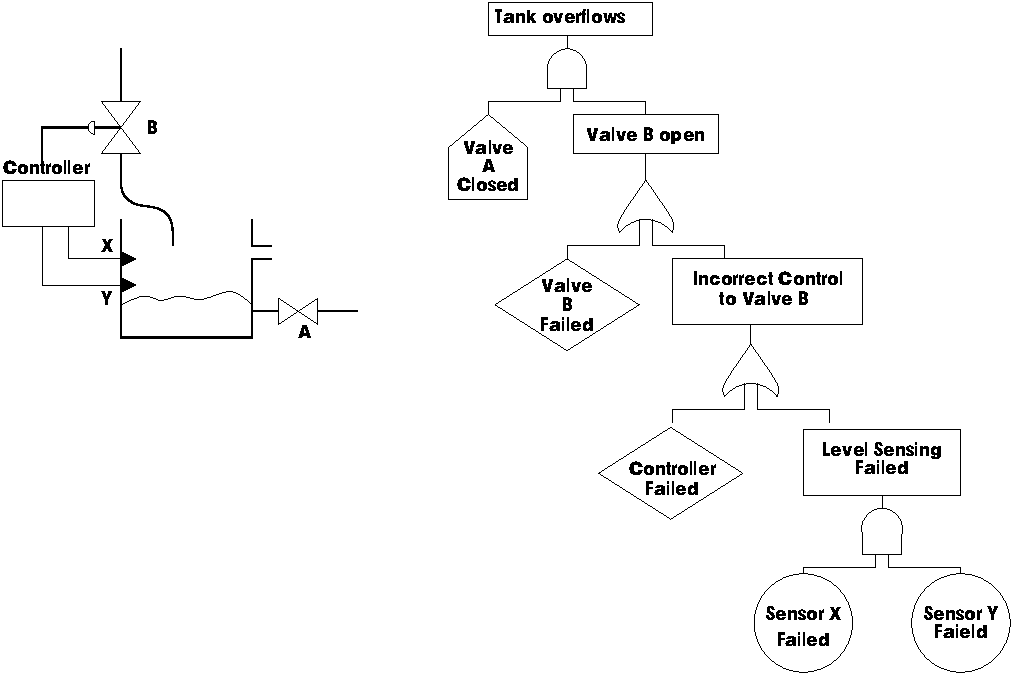
\includegraphics[scale=1.0]{\rootdir/safety/figures/fault-tree-valve}
\end{center}
\end{document}  


% LocalWords:  mins atomicity HAZOPS FMEA Therac Mulhouse Habsheim lp
% LocalWords:  ECUs counterfactuals lifecycle PHA HAZOP guideword
% LocalWords:  lcccc guidewords severities
